%%
%  ******************************************************************************
%  * #file    Szablon_raportu_EN_Latex.tex
%  * #author  Adrian Wójcik   adrian.wojcik(at)put.poznan.pl
%  *          
%  * #commit  Patryk Kościk   koscikpatryk(at)gmail.com
%  *          Modified the template for Projekt przejsciowy purposes          
%  *          
%  * #version 1.0
%  * #date    09-Mar-2022
%  * #brief   PROJPRZEJ
%  *
%  ******************************************************************************
%%  
\documentclass[11pt, a4paper]{article}

\usepackage{Szablon_raportu_EN_Latex}

% Wypełnijcie te dyrektywy zgodnie z waszym tematem
% \lab      -> NAZWA CZUJNIKA, np.: 'DHT22'
% \comment  -> Króciutki opis co to, np.: 'Cyfrowy budżetowy czujnik temperatury'
%
\lab{ULN2003}
\comment{Moduł sterownika do silników krokowych}
\author{Hubert Pietrzak}

% Absolutny zakaz dotykania tego tutaj bo jak dotkiecie to coś jebnie
\university{Politechnika Poznańska}
\faculty{Wydział Automatyki, Robotyki i Elektrotechniki}
\institute{Instytut Robotyki i Inteligencji Maszynowej}
\department{Zakład Sterowania i Elektroniki Przemysłowej}
\addbibresource{Szablon_raportu_EN_Latex.bib}
\nocite{*}


%%
%
% Początek dokumentu
%
%%
\begin{document}

%% Strona tytułowa %%
\mainpage{71460}
\newpage

\section*{Opis elementu} \addcontentsline{toc}{section}{Wstęp}

ULN2003 to uniwersalny sterownik silników krokowych. Umozliwia on proste sterowanie krokowymi silnikami z 4 fazami przy pomocy mikrokontrolera np. STM32 NUCLEO. Moduł umożliwia kontrolę kierunku obrotów i prędkości 4-fazowych silnków krokowych. Dedykowanym silnikiem do sterownika jest silnik krokowy 28BYJ, który zasilany jest 5V i ma on swój interfejs na płytce PCB. Sterownik jest wyposażony w wskaźnik stanu pracy poprzez wyświetlane Diody LED. Układ ma możliwość podłączenia napięcia zasilania do 12V. Część logiczna jest zasilana natomiast 5V.  Dodatkowo moduł jest wyposażony w IO porty, wejścia 1-4 są wykorzystywane do podłączenia pod mikrokontroler, z którego sterujemy silnikiem.

\vspace{0.5cm}
\begin{figure}[h]
\centering
\begin{subfigure}{.5\textwidth}
  \centering
  \includegraphics[width=.7\linewidth]{fig/obrazki/zdj_modułu/Temat.png}
  \caption{tylnia część modułu i ich wyprowdzenia}
  \label{fig:sub1}
\end{subfigure}%
\begin{subfigure}{.5\textwidth}
  \centering
  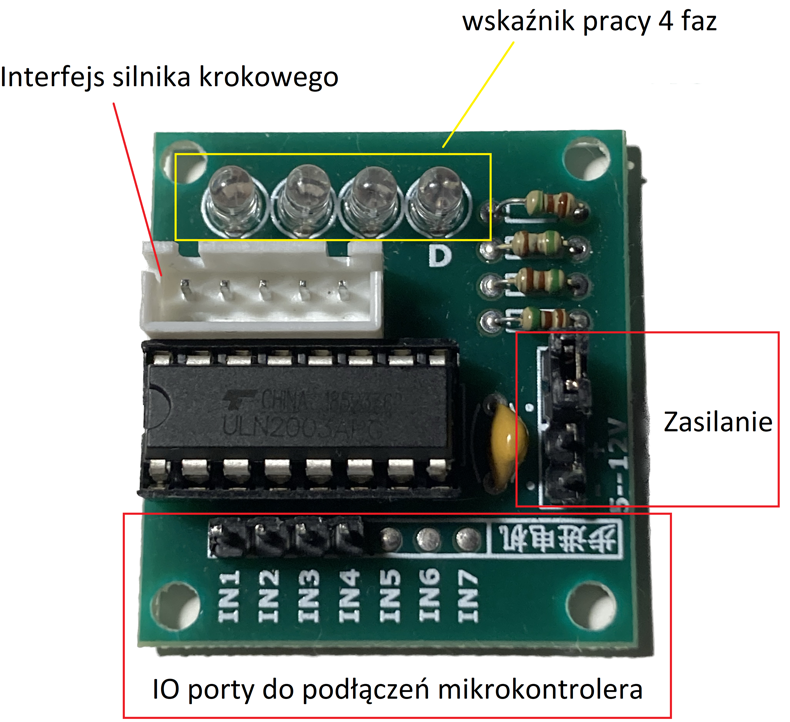
\includegraphics[width=.7\linewidth]{fig/obrazki/koncept.png}
  \caption{Opis elementów składowych sterownika}
  \label{fig:sub2}
\end{subfigure}
\caption{Wyprowadzenia ULN2003 i opis elementów modułu}
\label{fig:test}
\end{figure}
\vspace{0.5cm}

%\subsection{Zasada działania}


ULN2003APG to wysokonapięciowy, wysokoprądowy układ scalony składający się z siedmiu kanałów darlinghton NPN. Układ darlingtona to układ dwóch tranzystorów bipolarnych połączonych w jednej obudowie. Występują typy N-P-N jak i P-N-P. Kolektory w obu tranzystorach są połączone, a emiter pierwszego tranzystora jest połączony z bazą drugiego. Współczynnik wzmocnienia układu darlingtona jest równy iloczynowy wzmocnienia obu tranzystorów. W celu przyspieszania przełączania stosuje się dodatkowe rezystory.

\vspace{0.5cm}
\begin{figure}[h]
\centering
\begin{subfigure}{.5\textwidth}
  \centering
  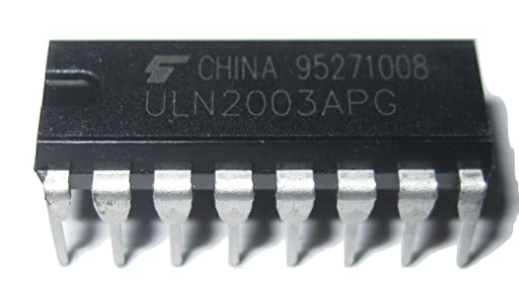
\includegraphics[width=.7\linewidth]{fig/obrazki/zasada_dzialania/uln3apg.png}  
  \caption{Układ scalony U2003APG}
  \label{fig:sub1}
\end{subfigure}%
\begin{subfigure}{.5\textwidth}
  \centering
  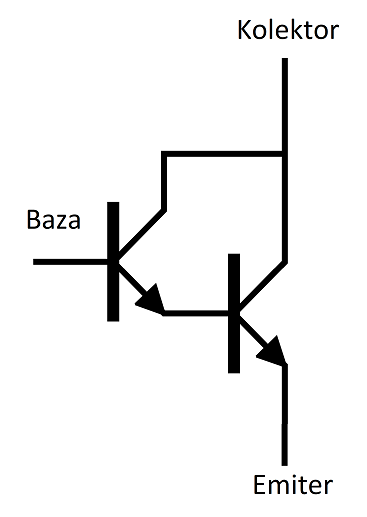
\includegraphics[width=.4\linewidth]{fig/obrazki/zasada_dzialania/darling2.png}
  \caption{Układ darlingtonowy typu N-P-N}
  \label{fig:sub2}
\end{subfigure}
\caption{Układ scalony U2003APG wraz z wykorzystywanym przez niego układem darlingtonowym}
\label{fig:test}
\end{figure}
\vspace{0.5cm}

%\subsection{Zastosowania}



\begin{figure}[h!]
    \centering
    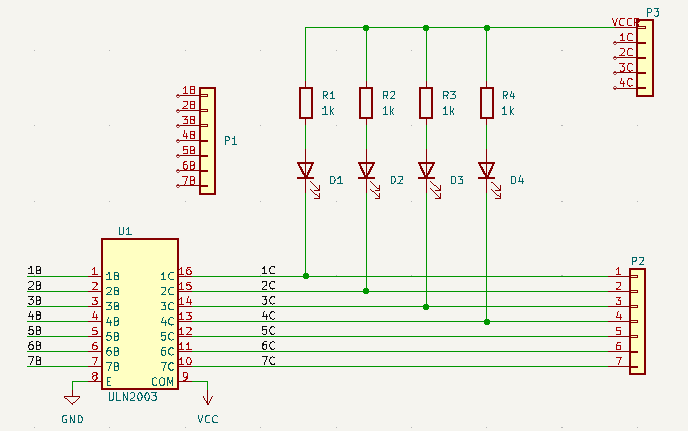
\includegraphics[width=0.99\textwidth]{fig/obrazki/działanie_ukladu/Schemat.png}
    \caption{Pełny schemat elektryczny sterownika}
    \label{fig:my_label}
\end{figure}





\newpage

%\section{Implementacja czujnika}


% \vspace{0.5cm}

% \vspace{0.5cm}
% \begin{figure}[h!]
%     \centering
%     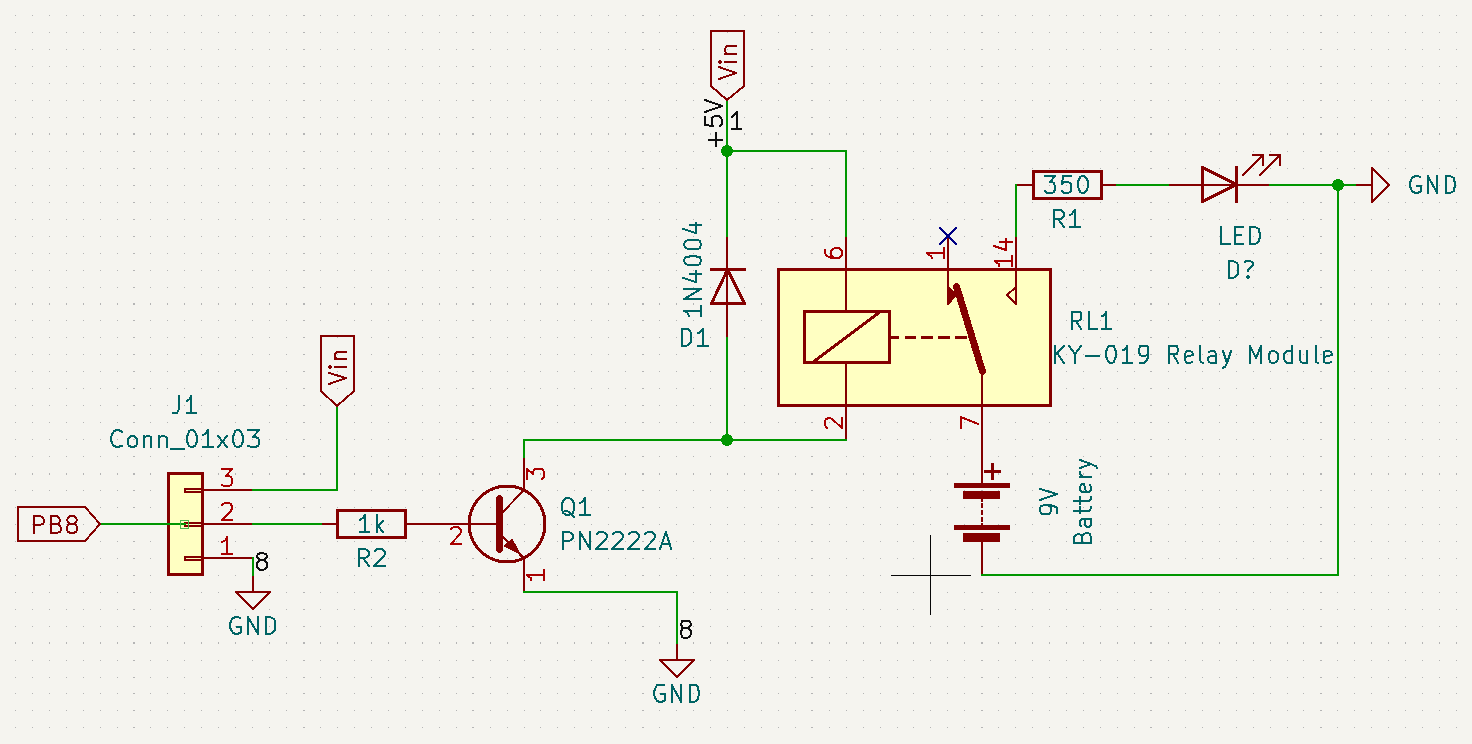
\includegraphics[scale=0.53]{fig/obrazki/polaczenie_modulu/Schematki.png}
%     \caption{Połaczenie elektryczne}
%     \label{fig:my_label}
% \end{figure}
% \vspace{0.5cm}


\newpage

%\section{Prezentacja działania układu}
\section{Użycie czujnika}

Poniższe zdjęcie \ref{fig:rysunek} prezentuje wykorzystanie modułu ULN2003 V2 jako pośrednika pomiędzy mikrokontrolerem, a silnikiem krokowym. Zasilanie +5v, sterowanie odbywa się za pomocą IO portów (4 przewody wychodzące po lewej stornie fotografii).Dodatkowo mamy białe złącze, stanowiące połączenie pomiędzy modułem sterującym, a silnikiem krokowym.
% \vspace{0.5cm}
% \begin{table}[h!]
%     \centering
%     \begin{tabular}{|c|c|c|c|} 
%         \hline
%         {NUCELO-F746ZG} & \multicolumn{2}{c|}{Moduł GY-320}  \\ 
%         \hline
%         Etykieta    &    Nr pinu &   Etykieta    \\ \hline
%         +3V3    &        1   &   VCC \\  \hline
%         GND     &      2   &   GND \\  \hline
%         PB9     &      3   &   SCL \\  \hline
%         PB6     &    4   &   SDA \\  \hline
%         - & 5 & ADDR\\ \hline
%     \end{tabular}
%     \caption{Połącznie pomiędzy modułem i mikrokontrolerem}
%     \label{tab:tab1}
% \end{table}

% W określonych chwilach czasowych (tutaj przykładowo 1 sekunda) dzięki pinowi sterującemu, przekazujemy (lub też nie) sygnał na wyjście przekaźnika, co obserwujemy zmieniającym się stanem zmiennej \textbf{RelayState}

\begin{figure}[h!]
    \centering
    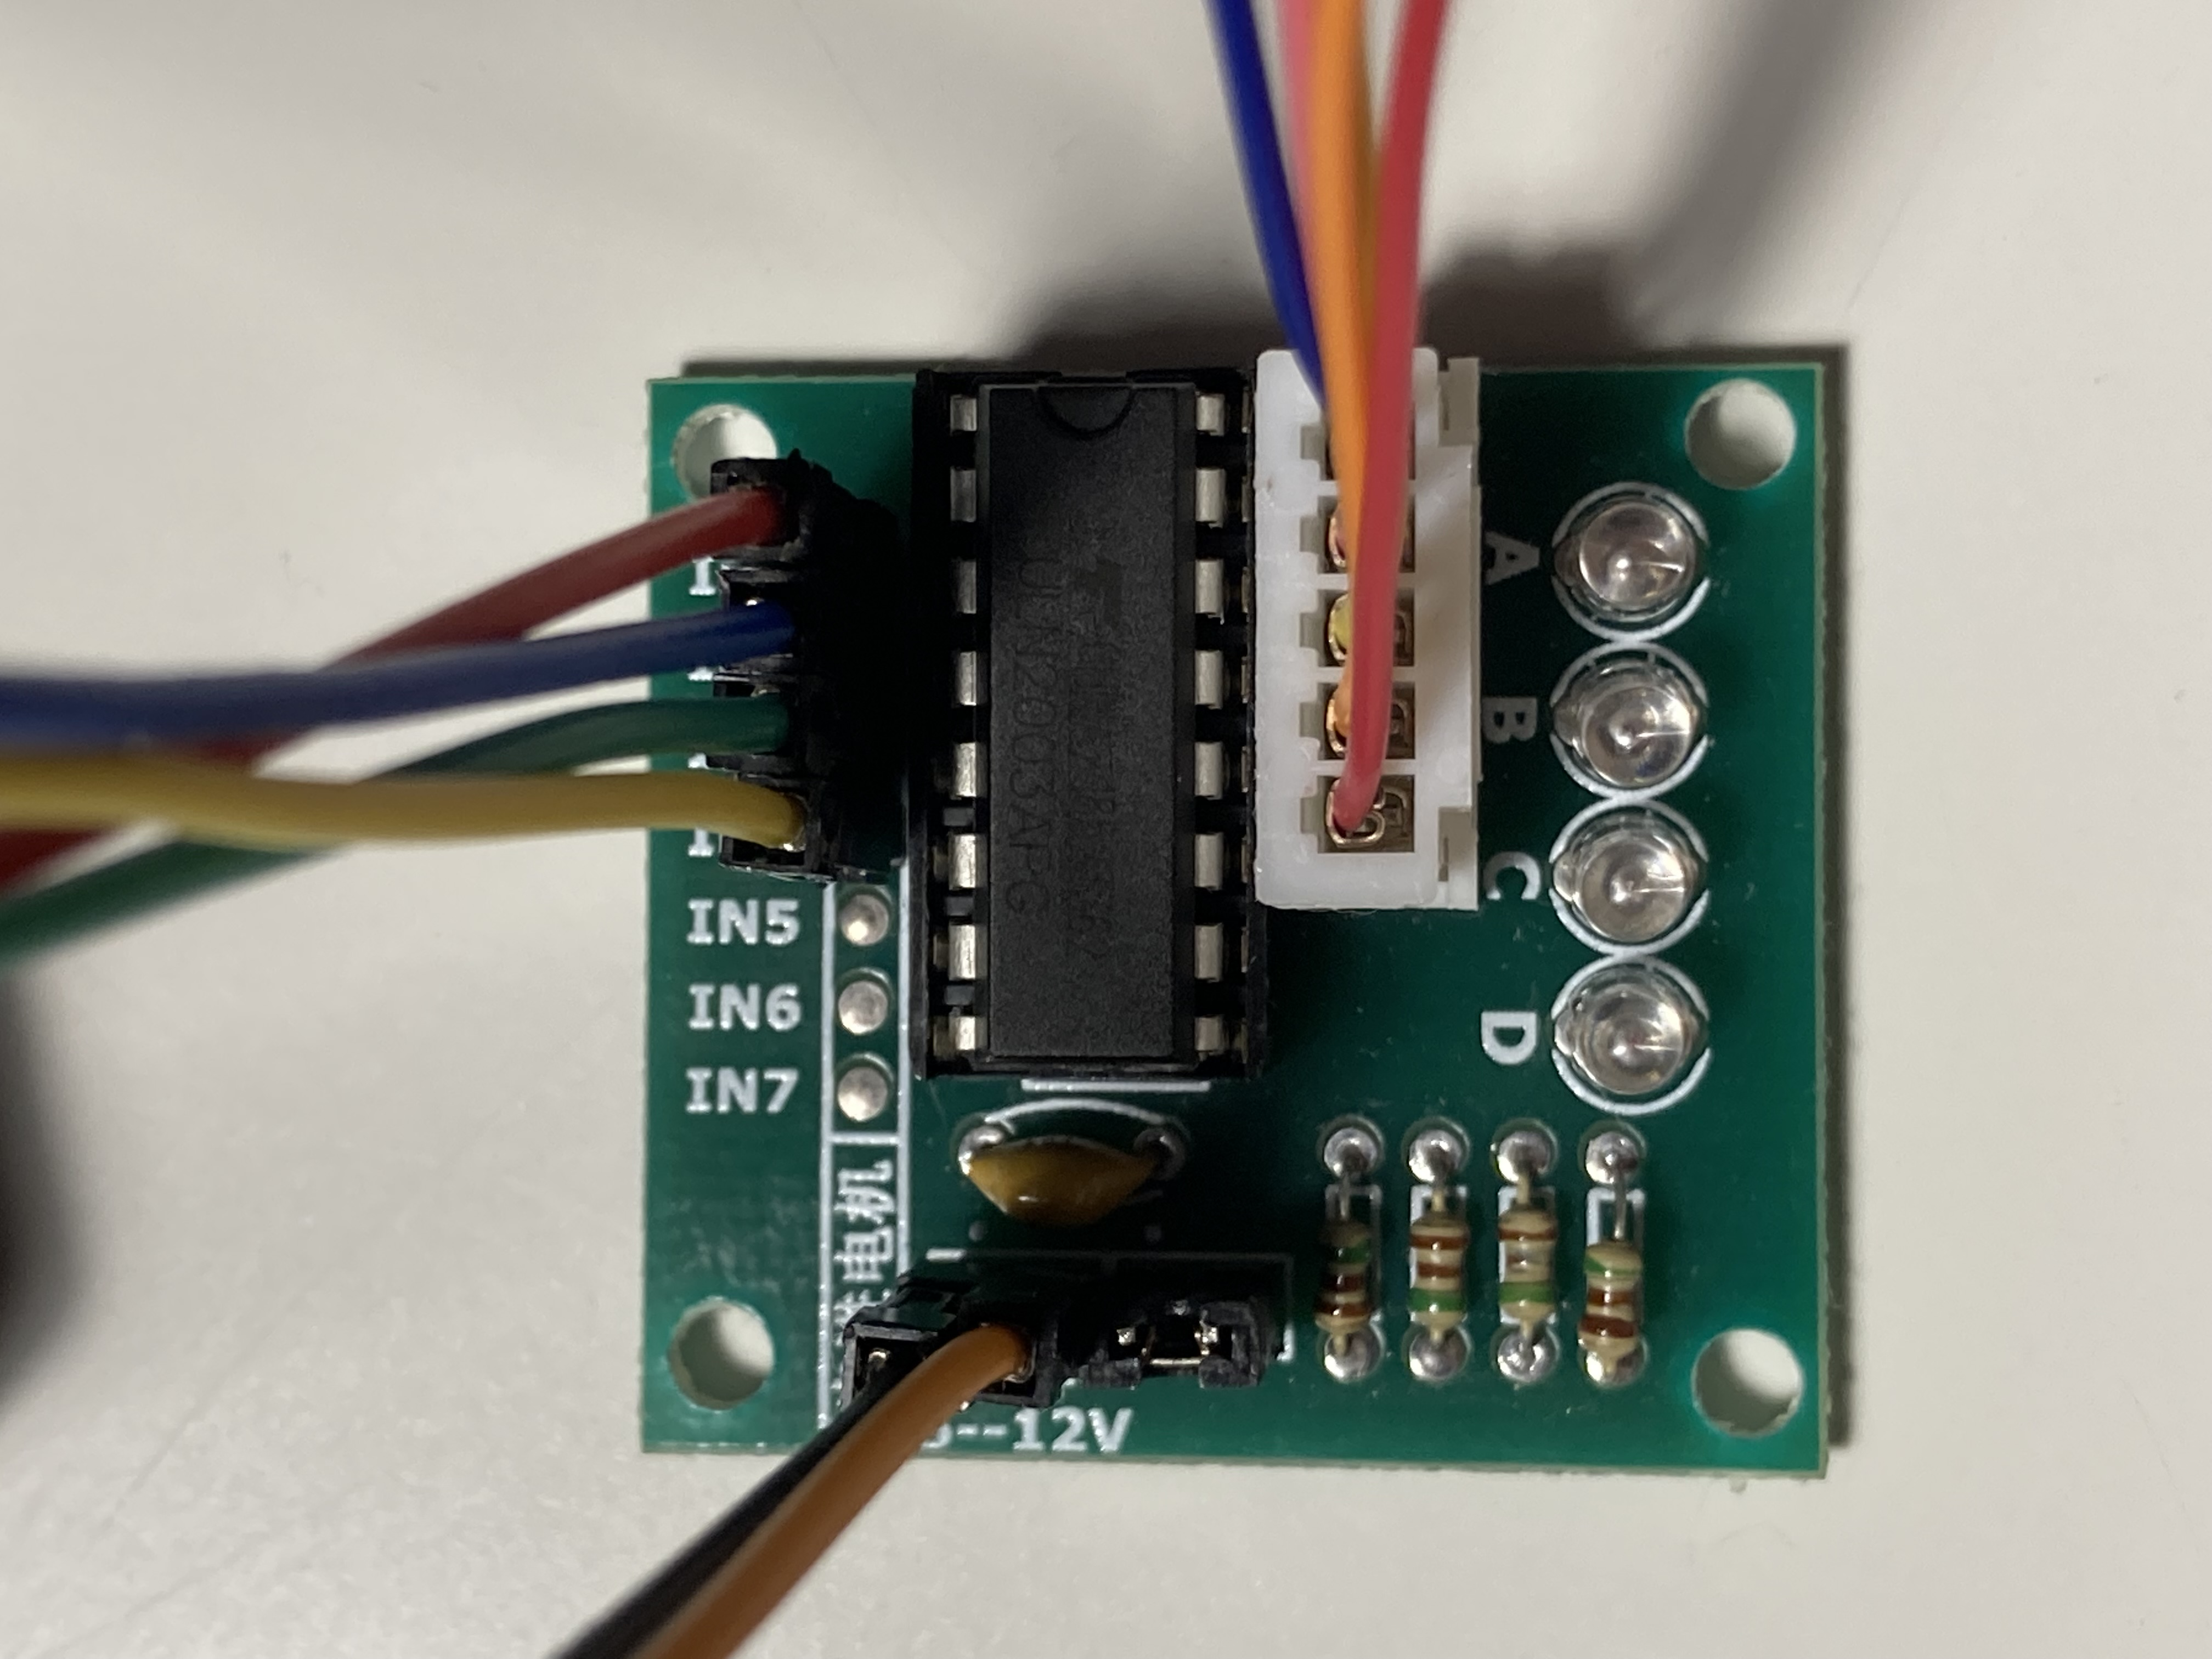
\includegraphics[scale=0.065]{fig/obrazki/działanie_ukladu/podlaczenie_blsiko.jpg}
    \caption{prawidłowe podłaczenie modułu sterownika silnika krokowego}
    \label{fig:rysunek}
\end{figure}

\vspace{0.5cm}
\begin{figure}[h!]
    \centering
    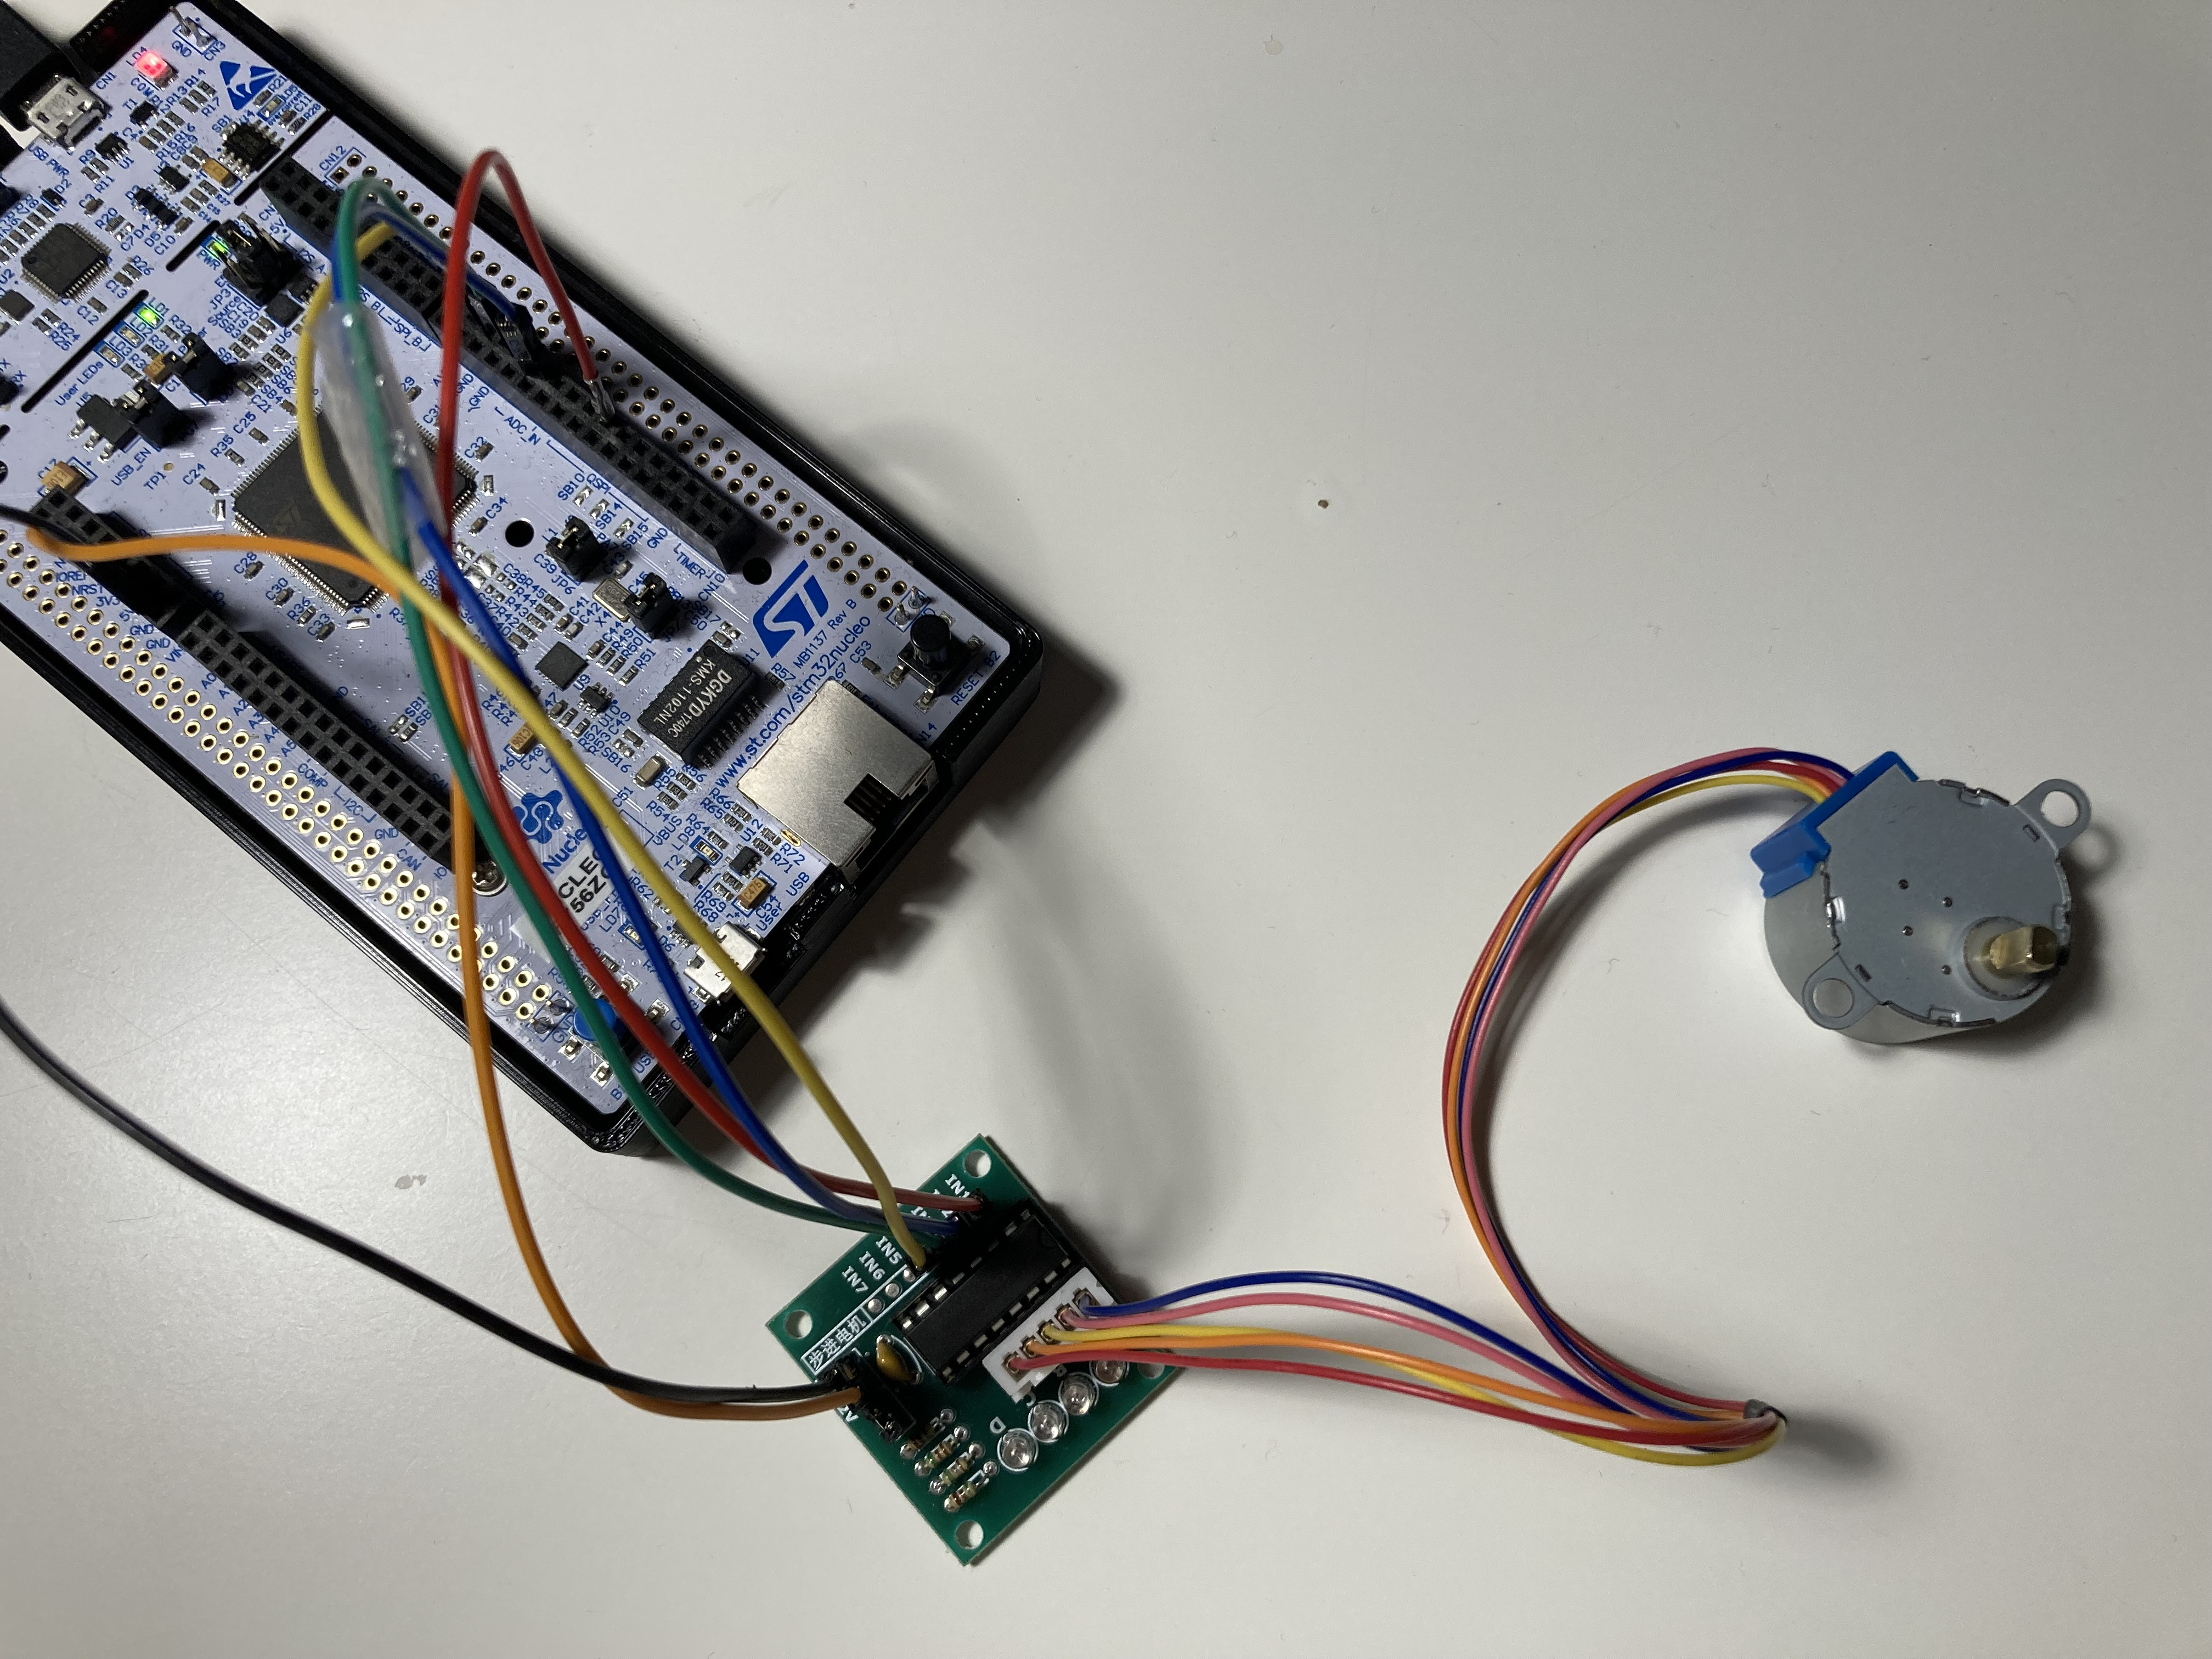
\includegraphics[scale=0.08]{fig/obrazki/działanie_ukladu/full.jpg}
    \caption{silnik krokowy sterowany przez moduł sterownika ULN2003 V2}
    \label{fig:my_label}
\end{figure}
\vspace{0.5cm}
Działanie modułu w aplikacji z mikrokontrolerem zostało zaprezentowane na materiale wideo zawartym w bibliografii % tu miejsce na odnosnik


% \vspace{0.5cm}
% \begin{figure}[h!]
%     \centering
%     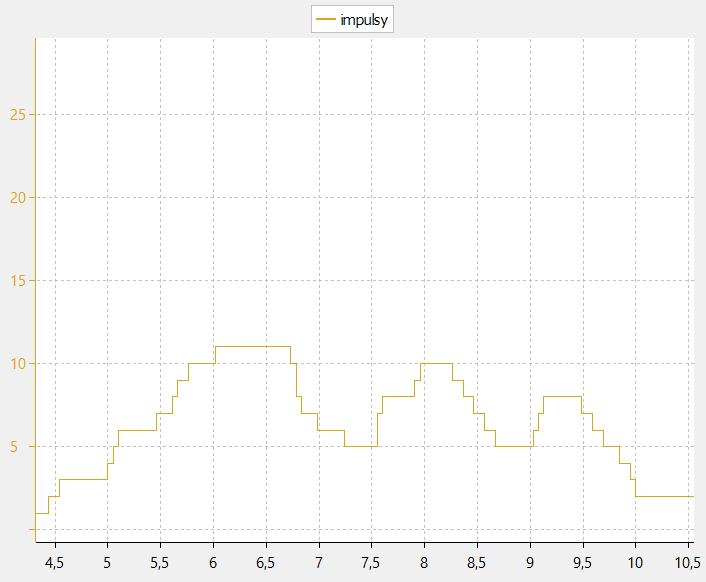
\includegraphics[scale=0.4]{fig/obrazki/działanie_ukladu/IMPULSY_PRZEBIEG.png}
%     \caption{Przebieg zmiany impulsów od czasu (obracanie enkoderem)}
%     \label{fig:my_label}
% \end{figure}
% \vspace{0.5cm}




\printbibliography[heading=bibintoc]

\end{document}